%==============================================================================
% Chapitre 55 - Structure d'une cartouche de chasse
%==============================================================================

\section{Introduction}

La cartouche de chasse moderne possède une architecture particulière qui
diffère sensiblement des cartouches métalliques utilisées dans les armes
rayées.

Elle est généralement constituée de plusieurs éléments superposés assurant
chacun une fonction spécifique.

\begin{aretenir}

Une cartouche de chasse est un système complet dans lequel chaque composant
participe aux performances du tir.

\end{aretenir}

\section{Vue d'ensemble}

Une cartouche de chasse moderne comprend généralement :

\begin{itemize}
    \item une douille ;
    \item une amorce ;
    \item une charge de poudre ;
    \item une bourre ;
    \item une charge de projectiles ;
    \item un sertissage.
\end{itemize}

\begin{figure}[htbp]
\centering

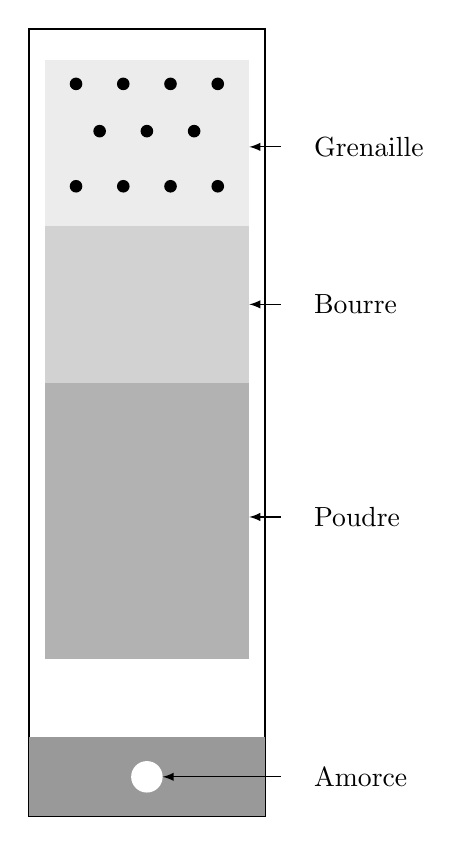
\begin{tikzpicture}[scale=1]

% Douille
\draw[thick] (0,0) rectangle (3,10);

% Grenaille
\fill[gray!15] (0.2,7.5) rectangle (2.8,9.6);

\foreach \x/\y in {
0.6/8.0,1.2/8.0,1.8/8.0,2.4/8.0,
0.9/8.7,1.5/8.7,2.1/8.7,
0.6/9.3,1.2/9.3,1.8/9.3,2.4/9.3
}
{
\fill (\x,\y) circle (0.08);
}

% Bourre
\fill[gray!35] (0.2,5.5) rectangle (2.8,7.5);

% Poudre
\fill[gray!60] (0.2,2.0) rectangle (2.8,5.5);

% Culot
\fill[gray!80] (0,0) rectangle (3,1);

% Amorce
\fill[white] (1.5,0.5) circle (0.2);

% Légendes
\node[right] at (3.5,8.5) {Grenaille};
\node[right] at (3.5,6.5) {Bourre};
\node[right] at (3.5,3.8) {Poudre};
\node[right] at (3.5,0.5) {Amorce};

\draw[-latex] (3.2,8.5) -- (2.8,8.5);
\draw[-latex] (3.2,6.5) -- (2.8,6.5);
\draw[-latex] (3.2,3.8) -- (2.8,3.8);
\draw[-latex] (3.2,0.5) -- (1.7,0.5);

\end{tikzpicture}

\caption{Coupe simplifiée d'une cartouche de chasse à grenaille.}
\label{fig:cartouche_chasse_grenaille}

\end{figure}

\section{La douille}

La douille constitue l'enveloppe principale de la cartouche.

Elle assure notamment :

\begin{itemize}
    \item le maintien des composants ;
    \item l'étanchéité des gaz ;
    \item l'alimentation de l'arme.
\end{itemize}

\section{Le culot métallique}

La partie inférieure de la cartouche comporte généralement un culot métallique.

Celui-ci renforce la zone soumise aux efforts les plus importants lors du tir.

\section{L'amorce}

L'amorce est située au centre du culot.

Elle initie la combustion de la poudre lorsque le percuteur la frappe.

\section{La poudre}

La poudre constitue la source d'énergie de la cartouche.

Sa combustion produit les gaz nécessaires à la propulsion de la charge.

\section{La bourre}

La bourre est un élément essentiel des cartouches de chasse.

Elle remplit plusieurs fonctions :

\begin{itemize}
    \item séparation de la poudre et des projectiles ;
    \item transmission de la poussée ;
    \item protection de la charge ;
    \item influence sur la gerbe.
\end{itemize}

\section{Les bourres traditionnelles}

Historiquement, les bourres étaient réalisées dans différents matériaux :

\begin{itemize}
    \item feutre ;
    \item carton ;
    \item fibres végétales.
\end{itemize}

\section{Les bourres modernes}

Les bourres modernes utilisent souvent des matériaux synthétiques.

Elles permettent un meilleur contrôle du comportement de la charge.

\begin{figure}[htbp]
\centering

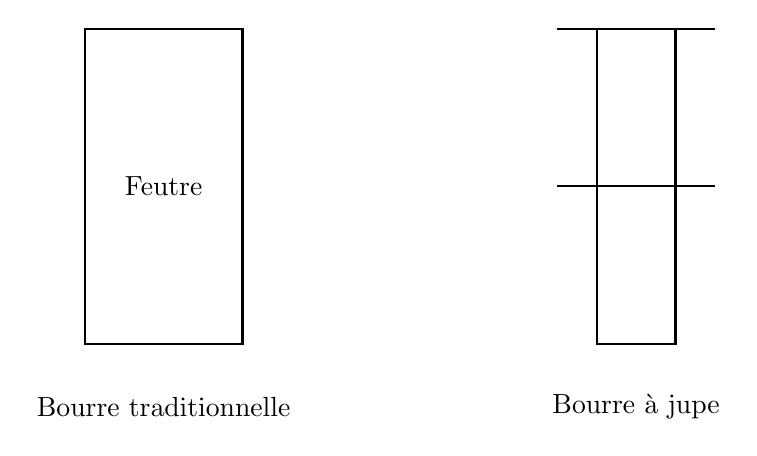
\begin{tikzpicture}[scale=1]

% Bourre feutre
\draw[thick] (0,0) rectangle (2,4);

\node at (1,2) {Feutre};

\node at (1,-0.8)
{Bourre traditionnelle};

% Bourre moderne
\begin{scope}[xshift=6cm]

\draw[thick] (0.5,0) rectangle (1.5,4);

\draw[thick] (0,2) -- (2,2);
\draw[thick] (0,4) -- (0.5,4);
\draw[thick] (1.5,4) -- (2,4);

\node at (1,-0.8)
{Bourre à jupe};

\end{scope}

\end{tikzpicture}

\caption{Exemple simplifié de bourres utilisées dans les cartouches de chasse.}
\label{fig:bourres_chasse}

\end{figure}

\section{La charge de projectiles}

Selon le type de munition, la charge peut être constituée :

\begin{itemize}
    \item d'une balle unique ;
    \item de chevrotines ;
    \item de grenaille.
\end{itemize}

\section{Le sertissage}

Le sertissage ferme l'extrémité avant de la cartouche.

Il assure le maintien de la charge avant le tir.

\section{Influence du sertissage}

Le sertissage influence notamment :

\begin{itemize}
    \item la pression ;
    \item la régularité ;
    \item le départ de la charge.
\end{itemize}

\begin{figure}[htbp]
\centering

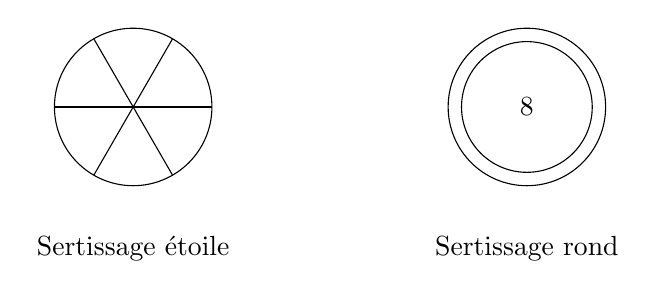
\begin{tikzpicture}[scale=1]

% Etoile
\draw (0,0) circle (1);

\foreach \a in {0,60,120,180,240,300}
{
\draw (0,0) -- (\a:1);
}

\node at (0,-1.8)
{Sertissage étoile};

% Rond
\begin{scope}[xshift=5cm]

\draw (0,0) circle (1);

\draw (0,0) circle (0.83);

\node at (0,0)
{8};

\node at (0,-1.8)
{Sertissage rond};

\end{scope}

\end{tikzpicture}

\caption{Exemples de sertissages couramment rencontrés.}
\label{fig:sertissages}

\end{figure}

\section{Longueur de la cartouche}

La longueur indiquée sur les cartouches de chasse correspond généralement à la
longueur après ouverture complète du sertissage.

Cette particularité peut surprendre les débutants.

\section{Compatibilité avec la chambre}

Une cartouche doit toujours être compatible avec la chambre de l'arme.

Le respect de cette compatibilité constitue une exigence de sécurité
fondamentale.

\section{Cartouches à grenaille}

Dans les cartouches à grenaille, la charge est constituée d'un grand nombre de
petits projectiles.

Leur organisation interne influence la qualité de la gerbe.

\section{Cartouches à balle}

Les cartouches à balle utilisent un projectile unique.

Leur structure générale reste néanmoins proche de celle des cartouches à
grenaille.

\begin{figure}[htbp]
\centering

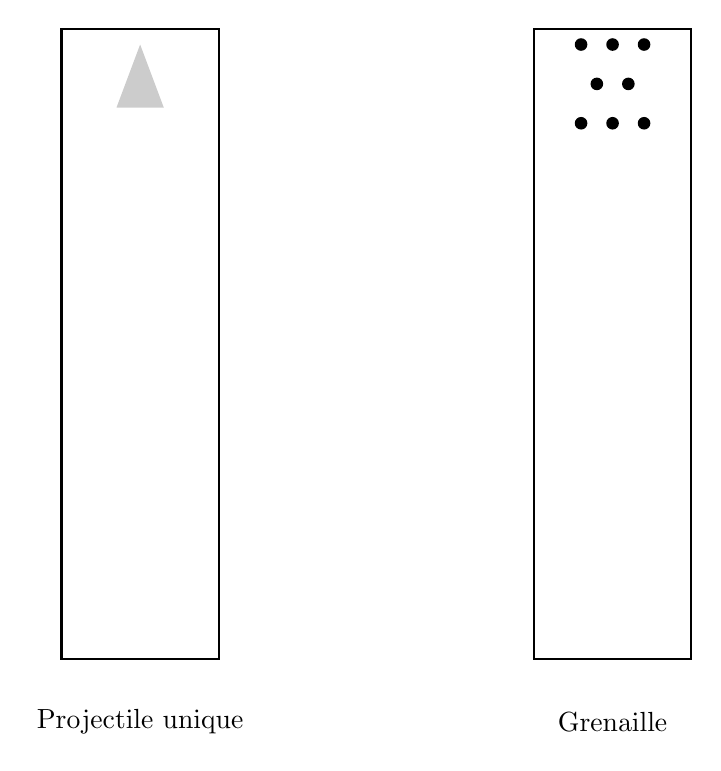
\begin{tikzpicture}[scale=1]

% Cartouche balle
\draw[thick] (0,0) rectangle (2,8);

\fill[gray!40]
(0.7,7)
--
(1,7.8)
--
(1.3,7)
--
cycle;

\node at (1,-0.8)
{Projectile unique};

% Cartouche grenaille
\begin{scope}[xshift=6cm]

\draw[thick] (0,0) rectangle (2,8);

\foreach \x/\y in {
0.6/6.8,1.0/6.8,1.4/6.8,
0.8/7.3,1.2/7.3,
0.6/7.8,1.0/7.8,1.4/7.8
}
{
\fill (\x,\y) circle (0.08);
}

\node at (1,-0.8)
{Grenaille};

\end{scope}

\end{tikzpicture}

\caption{Comparaison simplifiée entre une cartouche à balle et une cartouche à grenaille.}
\label{fig:balle_ou_grenaille}

\end{figure}


\section{Évolution des conceptions}

Les progrès des matériaux et des procédés industriels ont permis de faire
évoluer les cartouches de chasse tout en conservant leur architecture
générale.

\section{Vers les bourres et les chokes}

Parmi les composants d'une cartouche de chasse, la bourre joue un rôle
particulièrement important.

Les prochains chapitres examineront plus en détail son influence ainsi que
celle des chokes.

\section{À retenir}

\begin{aretenir}

\begin{itemize}
    \item Une cartouche de chasse est constituée de plusieurs éléments
          complémentaires.
    \item La bourre joue un rôle essentiel.
    \item Le sertissage influence le comportement de la cartouche.
    \item Les cartouches à balle et à grenaille partagent une architecture
          similaire.
    \item La compatibilité avec la chambre est indispensable.
\end{itemize}

\end{aretenir}
